\documentclass[10pt]{article}
\usepackage{tikz}
\usetikzlibrary{shapes.misc}
\usepackage[margin=0cm]{geometry}
\pagestyle{empty}
\tikzstyle{every node}=[cross out, draw, red]

\begin{document}

\vspace*{\fill}
\begin{center}
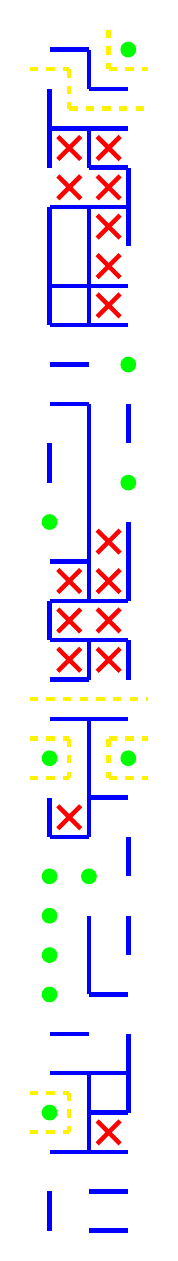
\begin{tikzpicture}[x=0.5cm, y=-0.5cm, ultra thick, blue]
% Walls
    \draw (0,0) -- (1,0);
    \draw (1,1) -- (2,1);
    \draw (0,2) -- (2,2);
    \draw (1,3) -- (2,3);
    \draw (0,4) -- (2,4);
    \draw (0,6) -- (2,6);
    \draw (0,7) -- (2,7);
    \draw (0,8) -- (1,8);
    \draw (0,9) -- (1,9);
    \draw (0,13) -- (1,13);
    \draw (0,14) -- (2,14);
    \draw (0,15) -- (2,15);
    \draw (0,16) -- (1,16);
    \draw (0,17) -- (2,17);
    \draw (1,19) -- (2,19);
    \draw (0,20) -- (1,20);
    \draw (1,24) -- (2,24);
    \draw (0,25) -- (1,25);
    \draw (0,26) -- (2,26);
    \draw (1,27) -- (2,27);
    \draw (0,28) -- (2,28);
    \draw (1,29) -- (2,29);
    \draw (1,30) -- (2,30);
    \draw (0,1) -- (0,3);
    \draw (0,4) -- (0,7);
    \draw (0,10) -- (0,11);
    \draw (0,14) -- (0,15);
    \draw (0,19) -- (0,20);
    \draw (0,29) -- (0,30);
    \draw (1,0) -- (1,1);
    \draw (1,2) -- (1,3);
    \draw (1,4) -- (1,7);
    \draw (1,9) -- (1,14);
    \draw (1,15) -- (1,16);
    \draw (1,17) -- (1,20);
    \draw (1,22) -- (1,24);
    \draw (1,26) -- (1,28);
    \draw (2,3) -- (2,5);
    \draw (2,9) -- (2,10);
    \draw (2,12) -- (2,14);
    \draw (2,15) -- (2,16);
    \draw (2,20) -- (2,21);
    \draw (2,22) -- (2,23);
    \draw (2,25) -- (2,27);
% Pillars
    \fill[green] (2,0) circle(0.2);
    \fill[green] (2,8) circle(0.2);
    \fill[green] (2,11) circle(0.2);
    \fill[green] (0,12) circle(0.2);
    \fill[green] (0,18) circle(0.2);
    \fill[green] (2,18) circle(0.2);
    \fill[green] (0,21) circle(0.2);
    \fill[green] (1,21) circle(0.2);
    \fill[green] (0,22) circle(0.2);
    \fill[green] (0,23) circle(0.2);
    \fill[green] (0,24) circle(0.2);
    \fill[green] (0,27) circle(0.2);
% Inner points in accessible cul-de-sacs
    \node at (0.5,2.5) {};
    \node at (1.5,2.5) {};
    \node at (0.5,3.5) {};
    \node at (1.5,3.5) {};
    \node at (1.5,4.5) {};
    \node at (1.5,5.5) {};
    \node at (1.5,6.5) {};
    \node at (1.5,12.5) {};
    \node at (0.5,13.5) {};
    \node at (1.5,13.5) {};
    \node at (0.5,14.5) {};
    \node at (1.5,14.5) {};
    \node at (0.5,15.5) {};
    \node at (1.5,15.5) {};
    \node at (0.5,19.5) {};
    \node at (1.5,27.5) {};
% Entry-exit paths without intersections
    \draw[dashed, yellow] (-0.5,0.5) -- (0.5,0.5);
    \draw[dashed, yellow] (1.5,0.5) -- (2.5,0.5);
    \draw[dashed, yellow] (0.5,1.5) -- (2.5,1.5);
    \draw[dashed, yellow] (-0.5,16.5) -- (2.5,16.5);
    \draw[dashed, yellow] (-0.5,17.5) -- (0.5,17.5);
    \draw[dashed, yellow] (1.5,17.5) -- (2.5,17.5);
    \draw[dashed, yellow] (-0.5,18.5) -- (0.5,18.5);
    \draw[dashed, yellow] (1.5,18.5) -- (2.5,18.5);
    \draw[dashed, yellow] (-0.5,26.5) -- (0.5,26.5);
    \draw[dashed, yellow] (-0.5,27.5) -- (0.5,27.5);
    \draw[dashed, yellow] (0.5,0.5) -- (0.5,1.5);
    \draw[dashed, yellow] (0.5,17.5) -- (0.5,18.5);
    \draw[dashed, yellow] (0.5,26.5) -- (0.5,27.5);
    \draw[dashed, yellow] (1.5,-0.5) -- (1.5,0.5);
    \draw[dashed, yellow] (1.5,17.5) -- (1.5,18.5);
\end{tikzpicture}
\end{center}
\vspace*{\fill}

\end{document}
